\chapter{Theoretical Background and Tools}
\label{chapter:Background}
This chapter describes algorithms and tools used in this project. It does not go into the details of each algorithm but it contains sufficient information to understand all the tools that we leveraged in interactive segmentation and recognition.
\section{Used Algorithms}
\subsection{RANSAC}
In order to explain the 3D features that were used as trackable parts of the point cloud in interactive segmentation for textuless objects basic understanding of RANSAC algorithm is needed. RANSAC stands for RAndom SAmple Consensus and it is an iterative algorithm that enables to find parameters of a mathematical model in the set of data containing outliers. The pseudocode of the algorithm is presented in Alg. \ref{alg:ransac}. 

\begin{algorithm}[htb!]
\While {$iterations < k$}
{
$maybe\_inliers$ := n randomly selected values from data
$maybe\_model$ := model parameters fitted to $maybe\_inliers$
$consensus\_set$ := $maybe\_inliers$

\ForEach {point in data not in $maybe\_inliers$}
{

\If {point fits $maybe\_model$ with an error $< t$}
{
add point to $consensus\_set$
}

}

\If {number of elements in $consensus\_set > d$}
{
(this implies that we may have found a good model,now test how good it is)\\
$this\_model$ := model parameters fitted to all points in $consensus\_set$\\
$this\_error$ := a measure of how well $this\_model$ fits these points\\



\If {$this\_error < best\_error$}
{            (we have found a model which is better than any of the previous ones,
            keep it until a better one is found)\\
            $best\_model$ := $this\_model$\\
            $best\_consensus\_set$ := $consensus\_set$\\
            $best\_error$ := $this\_error$\\
}


}
    increment iterations

}


\caption{RANSAC algorithm.}
  \label{alg:ransac}
\end{algorithm}

The most common example to explain RANSAC is a line fitting task in the 2D point dataset that contains outliers as shown in Fig. \ref{fig:ransac}. In the given dataset the algorithm would randomly pick two points and create a line equation that contains both of them. In the next step number of inliers is counted. Inliers meaning all the points that are lying within a certain threshold away from the line. If the number of inliers is bigger that the biggest number of inliers so far then it is saved. There are different implementation of RANSAC where the algorithm can run as long as there is not enough number of inliers or as the difference between them is becoming relatively small. As the result one obtains the best match to the given model that was found.

It is worth noticing that RANSAC algorithm can be used with many different models. In case of our system we use RANSAC to find the best fit to a line, a corner, a cylinder and a circle models. 



\begin{figure}
%\centering

{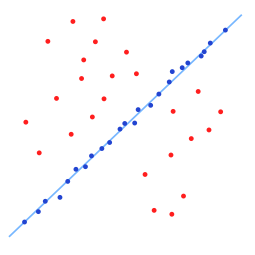
\includegraphics[width=0.5\columnwidth]{figures/ransac.png}}

\caption{RANSAC line fitting algorithm on an illustrative dataset.}
\label{fig:ransac}
\end{figure}



\subsection{3D and 2D Features}
As mentioned in the previous section RANSAC algorithm is the main tool used to extract 3D features on the objects. The differences between different geometric features that we are using is in the models used in RANSAC. We use a different mathematical representation of a feature, for example, a line or a cylinder, in order to extract it from the point cloud. 3D features are used only in the interactive segmentation of textureless objects part of the system. Our object recognition system employs various detectors and descriptors in the image space to extract and match 2D features.

In order to understand different 2D features that were used in our system it is crucial to be familiar with the concepts behind detectors, descriptors and matchers. We, as humans, have no problems in detecting distinctive features in the images we see. Moreover we can easily realize that there are some features in the image that we have seen before. To reproduce this process for an autonomous system there are multiple components needed since an image is seen by a computer as a simple set of pixel values without any high level meaning. First, the system has to detect points of interest in the image that are distinctive enough to find the same points multiple times. The algorithms that are behind this process are called detectors and their goal is to simply find good features. Having the region detected the next step is to describe the found features such that there is a big chance to find the same features later on under different conditions. The task of describing the found points belongs to a detector. In the next subsections we will describe different detector-descriptor pairs that were used in the object recognition part of the thesis.

\subsubsection{SIFT}
SIFT stands for Scale Invariant Feature Transform and is one of the most popular descriptor-detector pair. The SIFT detector    



\subsubsection{FAST and FREAK}


\subsection{Point Cloud Processing}
\subsubsection{Voxel Grid}
\subsubsection{Plane Estimation}
\subsubsection{Euclidean Clustering}

\subsection{Graph-based segmentation}
\subsection{Particle Filter}

\begin{itemize}
\item RANSAC
\item Particle Filter
\item 3d/2d features
\item Graph-based segmentation
\item Rigid body dynamics
\item Point cloud and point cloud processing
\end{itemize}


\section{Used Tools}
\begin{itemize}
\item Kinect
\item PR2
\item ROS
\item Gazebo
\item PCL
\item OpenCV
\end{itemize}






